\chapter{From SQL to Execution: the Catalyst Pipeline}
\label{ch:catalyst}

\begin{chapterintro}
A SQL string does not run. It is parsed into a tree, resolved against the
catalog, rewritten by rules, turned into a physical plan by choosing strategies,
and compiled to JVM bytecode. Every change you can make to a query's performance
is a change to one of those stages. This chapter traces the specimen query from
\Cref{ch:shape} through all of them and teaches you to read \texttt{EXPLAIN
FORMATTED} well enough to predict the physical plan before you run it.
\end{chapterintro}

\section{The pipeline, overview}
\label{sec:catalyst-overview}

Catalyst is the optimizer inside Spark SQL. It is a library for building and
rewriting trees, plus a fixed sequence of passes that turn a query into an
executable plan (\Cref{fig:catalyst-pipeline}). Every DataFrame operation and
every SQL statement goes through the same pipeline; the DataFrame API is just a
second front end that builds the same tree the SQL parser does.

\begin{figure}[htbp]
  \centering
  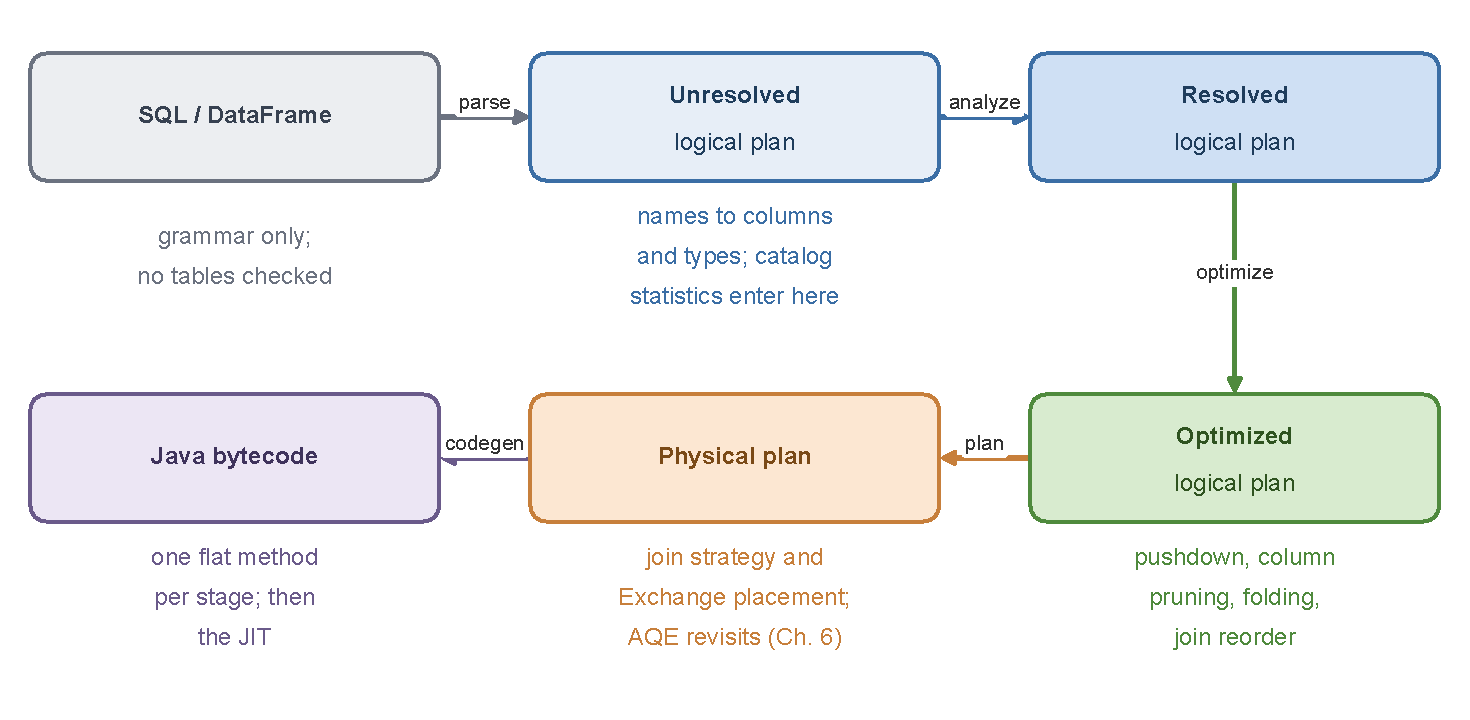
\includegraphics[width=\linewidth]{catalyst-pipeline.pdf}
  \caption{The compilation pipeline. Parsing produces a tree that is pure syntax.
  Analysis resolves names against the catalog. Logical optimization rewrites the
  tree with rules. Physical planning picks concrete operators and shuffle
  points. Code generation emits Java that the JIT compiles. The side notes name
  what each stage decides.}
  \label{fig:catalyst-pipeline}
\end{figure}

\begin{analogy}
Recall the kitchen from \Cref{sec:shape-driver}. The order goes through the same
five stages there as a query does here. A waiter writes the spoken order onto a
kitchen ticket in shorthand, without checking whether the kitchen actually has
those ingredients tonight --- that is \emph{parsing}: pure syntax. The expediter
then checks the ticket against the pantry and the menu, catching an order for a
dish that is not served or an ingredient that is out --- that is
\emph{analysis}, against the catalog. The head chef mentally simplifies the
prep --- ``we're already chopping onions for table 4, chop extra for this
ticket too'' --- without changing what gets served: that is \emph{logical
optimization}. Stations and techniques are then assigned --- grill or oven,
this cook or that one --- based on what is actually fastest tonight: that is
\emph{physical planning}. And a dish the kitchen has made a thousand times gets
cooked by hands that no longer think through each step: that is
\emph{whole-stage code generation} (\Cref{sec:wholestage-codegen}).
\end{analogy}

\begin{table}[H]
\centering\footnotesize
\renewcommand{\arraystretch}{1.2}
\begin{tabular}{@{}P{4.4cm}P{3.6cm}P{6cm}@{}}
\toprule
\textbf{In the kitchen} & \textbf{In Catalyst} & \textbf{What changes} \\
\midrule
waiter writes the ticket & parse & text $\to$ syntax tree; nothing checked \\
expediter checks the pantry \& menu & analyze & names resolved against the catalog \\
chef simplifies the prep & logical optimization & rule-based rewrites (\Cref{sec:catalyst-rules}) \\
stations \& techniques assigned & physical planning & operators \& shuffle points chosen \\
practiced hands, no thinking & whole-stage codegen & generated Java, then the JIT \\
\bottomrule
\end{tabular}
\caption{The analogy above, mapped exactly onto the pipeline in \Cref{fig:catalyst-pipeline}.}
\end{table}

Four representations matter, and you can print all of them (\Cref{sec:catalyst-explain}):

\begin{enumerate}
  \item the \textbf{unresolved logical plan} --- the parse tree; relations and
        columns are just names.
  \item the \textbf{resolved (analyzed) logical plan} --- names bound to real
        tables and typed columns.
  \item the \textbf{optimized logical plan} --- the same query, rewritten to do
        less work.
  \item the \textbf{physical plan} --- a tree of executable operators, with the
        shuffles made explicit as \emph{Exchange} nodes.
\end{enumerate}

The physical plan is what \Cref{ch:shape} called ``the plan.'' Reading it, and
knowing which pass produced each part of it, is what lets you look at a query and
say in advance how many stages it will have and where they will stall.

\section{Unresolved to resolved: the catalog}
\label{sec:catalyst-analysis}

The parser only checks grammar. \texttt{SELECT p.category FROM orders o JOIN
dim\_product p \dots} parses whether or not those tables exist; the result is a
tree whose relation and attribute nodes are still marked \emph{unresolved} ---
\texttt{orders} and \texttt{p.category} are held as names, not yet bound to
anything.

The \emph{analyzer} resolves them. It asks the \textbf{catalog} what
\texttt{orders} and \texttt{dim\_product} are, gets back their schemas, and
replaces each unresolved node with a concrete one: \texttt{category} becomes a
\texttt{string} column belonging to \texttt{dim\_product}, \texttt{delivery\_days}
becomes an \texttt{int} on \texttt{orders}, the \texttt{JOIN} condition is
type-checked, and \texttt{AVG(\dots)} is bound to the aggregate function. If a
name does not resolve, this is where the query fails --- before any work is
scheduled.

For Iceberg tables the catalog is a Spark \emph{catalog plugin}
(\Cref{ch:dsv2}); \Cref{ch:catalogs} covers
what it stores and how commits move through it. What matters here is that the
catalog is also where \emph{table statistics} come from --- row counts, column
value ranges, distinct counts. Spark's cost-based optimizer uses them to order
joins and to decide what is small enough to broadcast (\Cref{ch:joins}). An
Iceberg table exposes a total file size and row count from its metadata, but not
per-column statistics unless you have run \texttt{ANALYZE TABLE \dots COMPUTE
STATISTICS}. This is why so many lakehouse joins pick the wrong strategy at
planning time and have to be rescued by a hint or by AQE.

\section{Logical optimization: the rules that matter}
\label{sec:catalyst-rules}

The optimizer applies \emph{rules} --- functions from a logical plan to a better
logical plan --- grouped into \emph{batches} that run repeatedly until the plan
stops changing. Spark ships around a hundred rules. A handful account for most of
the speed-up, and all of them do the same thing: move work earlier, or delete it.

\paragraph{Predicate pushdown.} A filter is pushed as close to the scan as the
semantics allow, so fewer rows enter the rest of the plan. In the specimen the
\texttt{order\_ts} range moves into the \texttt{orders} scan, where it becomes a
\emph{partition filter} (Iceberg skips whole days) and a \emph{pushed filter}
(Parquet skips row groups). \Cref{ch:pruning} is about keeping this rule
working; a function or a \texttt{CAST} on the filtered column defeats it.

\paragraph{Column pruning.} The scan reads only the columns the query
references. The specimen touches \texttt{product\_id}, \texttt{delivery\_days},
\texttt{promised\_days}, and \texttt{order\_ts} from \texttt{orders} and
\texttt{product\_id}, \texttt{category} from \texttt{dim\_product} --- so a
fifty-column \texttt{orders} table is read four columns wide. A
\texttt{SELECT *} anywhere in a subquery turns this off.

\paragraph{Constant folding and simplification.} Expressions with no runtime
input are evaluated once at planning time; the \texttt{TIMESTAMP '2026-03-01
\dots'} literals are computed here, not per row. Boolean and null simplifications
(\texttt{x AND true}, \texttt{x = x}, \texttt{IS NOT NULL} on a non-nullable
column) are folded away.

\paragraph{Join reordering.} With reliable statistics and cost-based
optimization enabled (\conf{spark.sql.cbo.enabled} and
\conf{spark.sql.cbo.joinReorder.enabled}), a multi-way join is reordered to keep
intermediate results small --- join the pair that produces the fewest rows
first. Without statistics Spark keeps the written order, which is one more reason
Iceberg tables benefit from \texttt{ANALYZE}.

\begin{note}
Most optimizer rules are \emph{heuristic}: they rewrite the plan into a form
that is almost always better, using no cost model. Only join selection and join
reordering are cost-based, and only when statistics exist. When people say
``the optimizer is smart,'' they usually mean the heuristic rules, which are
reliable; the cost-based part is only as good as the catalog's numbers.
\end{note}

\section{What the rules are worth, measured}
\label{sec:catalyst-rules-measured}

The lab ran one query --- a three-day filter, a join of \texttt{orders} to
\texttt{dim\_product}, a constant expression \texttt{(1 + 0.05 + 0.02)} in the
aggregate --- and printed its plan at every stage with \texttt{EXPLAIN EXTENDED}.
Three rewrites are visible between the analyzed and the optimized plan:

\begin{lstlisting}[language=text,style=plan,caption={The same query before and after optimization (Spark 3.5.2; lines shortened)},captionpos=b,label=lst:catalyst-before-after]
== Analyzed Logical Plan ==
Aggregate [category], [category, sum(order_total * cast((1 + 0.05) + 0.02 as double)) AS gross]
+- Filter (order_ts >= 2026-03-05 AND order_ts < 2026-03-08 AND (1 = 1))
   +- Join Inner, (product_id = product_id)
      :- RelationV2[order_id, order_ts, product_id, customer_id, promised_days,
                    delivery_days, order_total] lab.db.orders
      +- RelationV2[product_id, category, list_price, title, brand, description] lab.db.dim_product

== Optimized Logical Plan ==
Aggregate [category], [category, sum(order_total * 1.07) AS gross]
+- Join Inner, (product_id = product_id)
   :- Filter isnotnull(product_id)
   :  +- RelationV2[order_ts, product_id, order_total] lab.db.orders
   +- Filter isnotnull(product_id)
      +- RelationV2[product_id, category] lab.db.dim_product
\end{lstlisting}

Read the differences line by line. The constant expression became the literal
\texttt{1.07} (constant folding), and \texttt{1 = 1} vanished. Both scans shrank from
seven and six columns to three and two (column pruning). The date predicate left
the \texttt{Filter} --- it was pushed into the scan, where
\Cref{sec:dsv2-pushdown} shows it is fully handled because three whole days align
with the partitions --- and the optimizer added \conf{isnotnull(product_id)}
filters, inferred from the inner-join condition, which cannot change the result and
let the scan discard null keys early.

To price each rule, the lab re-ran the query with one rule excluded at a time
through \conf{spark.sql.optimizer.excludedRules}
(\Cref{fig:optimizer-rules-measured}). The result is identical in every run; only
the work changes.

\begin{figure}[htbp]
  \centering
  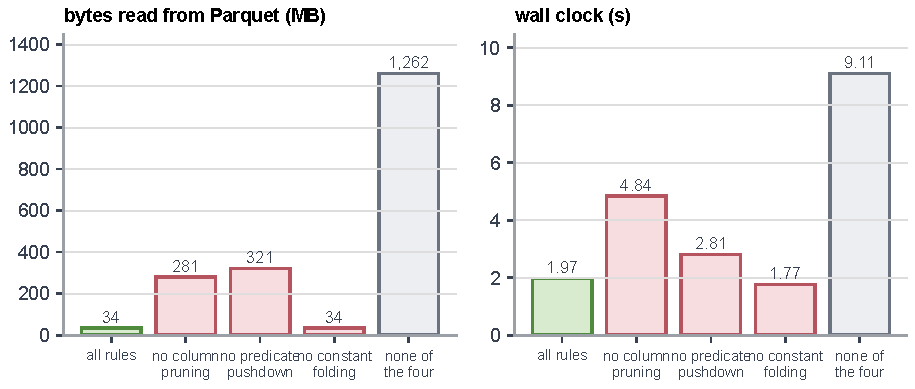
\includegraphics[width=\linewidth]{optimizer-rules-measured.pdf}
  \caption{Bytes read and wall clock with one optimizer rule excluded. Without
  column pruning the scan read 8$\times$ the bytes (281 against 34~MB); without
  predicate pushdown it read 321~MB and 32 million rows instead of 4.9 million; with
  all three rules excluded together, 1,262~MB and 9.1~s against 34~MB and 2.0~s. Excluding constant folding changed neither bytes nor time here: the
  folded expression was cheap next to the scan.}
  \label{fig:optimizer-rules-measured}
\end{figure}

Two cautions from the experiment. Excluding the Iceberg scan-pushdown rule by name
changed nothing --- bytes and rows were identical to the baseline --- so that rule
is not removable this way, and its effect is the one measured in
\Cref{fig:pushdown-rows-by-predicate} instead. And wall-clock times of 1--2 seconds
carry run-to-run noise of the order of the differences between the
constant-folding and baseline bars; the byte and row counts are the reliable
column.

\section{Physical planning and strategies}
\label{sec:catalyst-physical}

The optimized \emph{logical} plan still says only \emph{what} to compute. The
planner turns each logical operator into one or more \emph{physical} operators by
applying \emph{strategies}:

\begin{itemize}
  \item a logical \texttt{Join} becomes \conf{BroadcastHashJoin},
        \conf{ShuffledHashJoin}, or \texttt{SortMergeJoin}, chosen from the
        estimated sizes of its inputs and \conf{spark.sql.autoBroadcastJoinThreshold}
        (\Cref{ch:joins}).
  \item a logical \texttt{Aggregate} becomes a partial \texttt{HashAggregate} on
        each partition, an \texttt{Exchange} to bring equal keys together, and a
        final \texttt{HashAggregate}.
  \item a logical \texttt{Sort} that needs a global order becomes a
        range-partitioning \texttt{Exchange} followed by a local \texttt{Sort}.
\end{itemize}

The two-phase aggregate is worth tracing through with actual row counts,
because "partial then final" only pays off if the partial step actually
shrinks the data. Say the specimen's \texttt{orders} scan is split across 200
partitions, and category \texttt{electronics} has rows scattered across all
of them. The \emph{partial} \texttt{HashAggregate} runs once per partition,
independently, before any data moves: partition 17 might hold 40,000
\texttt{electronics} rows and collapse them to a single
\texttt{(electronics, count=40000, sum=\ldots)} row; partition 84 does the
same for its own share. Every partition now emits at most one row per
category it happened to contain --- typically a few dozen rows instead of
tens of thousands. The \texttt{Exchange} then shuffles only \emph{those}
small partial rows by category, and the \emph{final} \texttt{HashAggregate}
combines the (now few hundred, not tens of millions) partial results into
one row per category. The shuffle moves kilobytes of pre-aggregated rows
instead of gigabytes of raw ones --- that reduction is the entire reason the
planner inserts a partial stage at all rather than shuffling raw rows
straight to one final aggregate.

The planner also inserts \texttt{Exchange} (shuffle) and \texttt{Sort} nodes
wherever an operator's required input distribution is not already satisfied ---
and, crucially, \emph{removes} them where it is. If two joins share a key and the
data is already partitioned by it, the second join reuses the first's exchange.
This is why the \emph{number of Exchange nodes in the physical plan} is the
single best predictor of a query's cost, and why \Cref{ch:shape} told you to
count them in the UI.

For the specimen, the planner produces (captured on the lab of
\Cref{sec:refenv-lab}): two scans, each followed by an \texttt{Exchange
hashpartitioning(product\_id, 200)}; a \texttt{SortMergeJoin}, because
\texttt{dim\_product} is about 170~MB, far over the 10~MB broadcast threshold
--- Iceberg reports a table's size from its snapshot metadata, so the planner
knows this without any column statistics; a partial \texttt{HashAggregate}; a
second exchange, \texttt{hashpartitioning(category, 200)}, because the aggregate
groups by a different key than the join, so the join's partitioning does not
carry over; the final \texttt{HashAggregate}; and a fourth exchange,
\texttt{rangepartitioning(on\_time\_rate, 200)}, for the global \texttt{ORDER BY}
before the final \texttt{Sort}. Four exchanges, so five stages, as
\Cref{fig:job-stage-task} shows.

\section{Whole-stage code generation}
\label{sec:wholestage-codegen}

A physical plan could be executed by walking the operator tree and calling
\texttt{next()} on each node once per row --- the ``Volcano'' iterator model. For
a chain of \texttt{Filter} $\to$ \texttt{Project} $\to$ \texttt{HashAggregate},
every row passes through three virtual method calls, and the boxing and the
short-lived row objects between operators usually cost more than the actual
filtering and arithmetic.

Spark does not do this. For a chain of operators within a stage it \emph{generates
Java source} for the whole chain --- one method that scans, filters, projects,
and feeds the aggregate in a tight loop, with no virtual call, no intermediate
row object, and field access straight out of the packed binary row
(\Cref{ch:tungsten}). That method is compiled to bytecode and then by the JVM's
JIT to native code.

In a printed plan you see this as a numbered marker. Operators fused into one
generated function are wrapped: \texttt{*(2) HashAggregate}, \texttt{*(2)
Project}, \texttt{*(2) Filter}. The \texttt{*(n)} means ``part of generated stage
\texttt{n}''; the number is just a sequential id, not an execution order. An
operator \emph{without} a star is a boundary where fusion stopped and Spark falls
back to row-at-a-time.

A stage stops being generated for a handful of reasons, and a plan missing stars
where you expect them is usually hitting one:

\begin{itemize}
  \item an \texttt{Exchange} or \conf{BroadcastExchange} --- you cannot fuse
        operators across a network boundary, so codegen always restarts on the
        far side of a shuffle;
  \item a stage whose input or output schema has more columns than
        \conf{spark.sql.codegen.maxFields} (100 by default);
  \item a generated method that would exceed the JVM's 64\,KB bytecode limit for
        a single method (\conf{spark.sql.codegen.hugeMethodLimit}); Spark logs
        \texttt{Found too long generated codes} and drops that stage to the
        interpreter;
  \item a compile failure in the generated Java, after which Spark silently falls
        back (\conf{spark.sql.codegen.fallback}) --- the only trace is a
        \texttt{WARN} in the executor log;
  \item an imperative (non-declarative) aggregate or UDAF. Spark's built-in
        aggregates (\texttt{SUM}, \texttt{AVG}, \texttt{COUNT}) are
        \emph{declarative}: each is expressed as a small set of Catalyst
        expressions (an update expression, a merge expression) that the
        codegen framework can inline directly into the generated method, the
        same as any other expression. A UDAF written against the older
        imperative \texttt{Aggregator}/\conf{UserDefinedAggregateFunction}
        API instead hands Spark opaque Scala/Java method bodies to call ---
        there is no expression tree to inline, so Spark can only invoke those
        methods the ordinary virtual-call way, and fusion stops at that node.
\end{itemize}

A plan missing a star where you expected one confirms which of these fired.
Compare a healthy plan, \texttt{*(2) HashAggregate(keys=[category], \ldots)},
against the same query with an imperative UDAF substituted in for the
\texttt{AVG}: the node becomes plain \texttt{HashAggregate(keys=[category],
\ldots)} with no leading \texttt{*}, and every operator that would otherwise
have fused with it in that stage loses its star too, since fusion is
all-or-nothing for the chain that touches the un-fusable node.

\texttt{EXPLAIN CODEGEN} prints the generated Java for every whole-stage stage,
which is how you confirm what actually got fused.

\section{Reading \texttt{EXPLAIN}}
\label{sec:catalyst-explain}

Now that you know what the \texttt{*(n)} markers and \texttt{Exchange} nodes
mean, here is how to read the rest of a plan systematically.
\texttt{EXPLAIN} prints the plans without running the query. There are five modes,
selected by a keyword in SQL or a \texttt{mode} argument to
\texttt{df.explain(\ldots)}; \Cref{tab:catalyst-explain-modes} lists them.

\begin{table}[htbp]
\centering\footnotesize
\renewcommand{\arraystretch}{1.15}
\begin{tabular}{@{}P{2.7cm}P{11.2cm}@{}}
\toprule
\textbf{Mode} & \textbf{Shows} \\
\midrule
(default) & the physical plan only --- the quick check for join strategy, shuffle count, codegen \\
\texttt{EXTENDED} & all four plans: parsed, analyzed, optimized logical, and physical --- use to see what a rule did \\
\texttt{FORMATTED} & the physical plan as a compact tree \emph{plus} a numbered list expanding each node's detail --- the one to learn \\
\texttt{COST} & the optimized logical plan annotated with the planner's row-count and size \emph{estimates} --- use to see why it did not broadcast \\
\texttt{CODEGEN} & the physical plan plus the generated Java for each whole-stage stage \\
\bottomrule
\end{tabular}
\caption{The \texttt{EXPLAIN} modes. Start with the default for a quick check and
move to \texttt{FORMATTED} when you need each node's detail.}
\label{tab:catalyst-explain-modes}
\end{table}

\texttt{EXPLAIN FORMATTED} has two parts: a compact tree, then a numbered list
where each node's details are spelled out. Read the tree \textbf{bottom-up} ---
the leaves are scans, the root is the final operator.

\begin{lstlisting}[language=text,numbers=none,style=plan,caption={\texttt{EXPLAIN FORMATTED} on the specimen, before it runs (trimmed)},captionpos=b,label=lst:explain-anatomy]
== Physical Plan ==
AdaptiveSparkPlan (17)
+- Sort (16)                         -- global ORDER BY
   +- Exchange (15)                  -- range(on_time_rate): shuffle #4
      +- HashAggregate (14)          -- final aggregate
         +- Exchange (13)            -- hash(category): shuffle #3
            +- HashAggregate (12)    -- partial aggregate
               +- Project (11)
                  +- SortMergeJoin Inner (10)   -- dim_product: too big
                     :- Sort (5)               -- local sort per input
                     :  +- Exchange (4)        -- hash(product_id): #1
                     :     +- Project (3)
                     :        +- Filter (2)
                     :           +- BatchScan lab.db.orders (1)
                     +- Sort (9)
                        +- Exchange (8)        -- hash(product_id): #2
                           +- Filter (7)
                              +- BatchScan lab.db.dim_product (6)

(1) BatchScan lab.db.orders
    Output [4]: [order_ts, product_id, promised_days, delivery_days]
    filters=order_ts IS NOT NULL, order_ts >= 1772323200000000,
            order_ts < 1772928000000000, product_id IS NOT NULL
\end{lstlisting}

The \texttt{*(n)} markers appear only after execution, in the final plan; the
plan before it runs has none. The root is \conf{AdaptiveSparkPlan} because AQE
is on (\Cref{ch:aqe}).

The nodes you will meet most --- a full catalogue is \Cref{app:plans}:

\paragraph{Scan, at every leaf.} \texttt{BatchScan} for an Iceberg or other
DataSource~V2 table (Spark's newer, pluggable table-source API, covered in
\Cref{ch:dsv2} --- Iceberg tables always go through it); \texttt{FileScan
parquet} for a Hive-catalogued table;
\conf{InMemoryTableScan} for cached data. Its fields are where pruning is
confirmed or denied (an Iceberg \texttt{BatchScan} prints its pushed predicates in
one \texttt{filters=} list instead, as above): \conf{PartitionFilters} (whole partitions skipped ---
directories on object storage), \texttt{PushedFilters} (row groups skipped inside
the files that are read, using column min/max and bloom filters),
\texttt{DataFilters} (everything, including the part evaluated row-by-row after
reading), and \texttt{ReadSchema} (the columns actually read --- should be only
those the query needs). \texttt{Batched: true} means vectorized columnar reads
are on.

\paragraph{Exchange, at every stage boundary.} Each \texttt{Exchange} is one
shuffle: serialize, write to local disk, transfer, re-read. Count them --- it is
the best single predictor of cost. \texttt{hashpartitioning(key, n)} co-locates
equal keys (joins, \texttt{GROUP BY}); \conf{rangepartitioning} produces
globally ordered partitions (a global \texttt{ORDER BY}); \conf{SinglePartition}
funnels everything to one task (a global aggregate, \texttt{coalesce(1)}). The
\conf{ENSURE_REQUIREMENTS} tag means the planner inserted this exchange because
a downstream operator needs that distribution. \conf{BroadcastExchange} is a
different move: it ships one small side whole to every executor, and it appears
only below the build side of a \conf{BroadcastHashJoin}.

\paragraph{Sort.} \texttt{Sort [key ASC NULLS FIRST], false, 0} --- the boolean
is \texttt{true} for a global sort, \texttt{false} for a local per-partition one.
A \texttt{SortMergeJoin} always has two local sorts, one per input, between the
exchanges and the join.

\begin{tip}
The fast scan of any plan, in order: (1) the join operator ---
\texttt{SortMergeJoin} on a table you expected to be small means its size
estimate is over the broadcast threshold (\Cref{ch:joins}); (2) the number of \texttt{Exchange} nodes; (3)
\conf{PartitionFilters} non-empty on a partitioned table (\Cref{ch:pruning});
(4) \texttt{PushedFilters} non-empty; (5) \texttt{ReadSchema} listing only needed
columns.
\end{tip}

After the query runs, the SQL tab shows the same tree with \emph{actual} row
counts and, if AQE was active, the adapted plan rooted at
\texttt{AdaptiveSparkPlan isFinalPlan=true} --- which is the plan that really ran,
not the one \texttt{EXPLAIN} printed beforehand (\Cref{ch:aqe}).

\section{Summary}
\label{sec:catalyst-summary}

A query becomes an execution in fixed stages: parse to a syntax tree, resolve
names and types against the catalog, rewrite the logical plan with mostly
heuristic rules (pushdown, column pruning, folding; join reordering only with
statistics), choose physical operators and shuffle points with strategies, and
generate Java for each pipelined chain. The physical plan --- readable with
\texttt{EXPLAIN FORMATTED} --- tells you the join strategy, the number of
shuffles, and whether pruning and column selection are working, which together
determine how many stages the query has and where it will spend its time. The
recurring lakehouse failure is missing catalog statistics, which makes the
cost-based decisions (join strategy and order) unreliable until you
\texttt{ANALYZE} or override.

\exercisehead
\begin{exercises}
\item Run \texttt{EXPLAIN FORMATTED} on the specimen query. Confirm the two
      Exchange nodes, the \texttt{SortMergeJoin}, and a non-empty
      \conf{PartitionFilters} on the \texttt{orders} scan.
\item Write the same result three ways: with an explicit subquery, with a CTE,
      and as one flat statement. Compare the \emph{optimized} logical plans.
      Which differ, and which are identical?
\item Add \texttt{WHERE CAST(o.product\_id AS STRING) = '47'} to the query and
      re-run \texttt{EXPLAIN FORMATTED}. What happened to \texttt{PushedFilters}?
\end{exercises}
